\documentclass[12pt,a4paper]{article}
%%% Packages %%%
\usepackage{algorithm}		% Algorithms with captions (\begin{algorithm}).
\usepackage{algpseudocode}	% Algorithm pseudocode (\begin{algorithmic}).
\usepackage{amsfonts} 		% For extra mathy stuff (\mathbb).
\usepackage{amsmath} 		% For section headers.
\usepackage{amssymb} 		% For extra mathy stuff, e.g. \therefore.
\usepackage{amsthm}  		% Custom theorem styles.
\usepackage[toc,page]{appendix} % Appendices.
\usepackage{array} 			% Special tabular.
\usepackage{braket} 		% For \set \bra \ket commands.
\usepackage{caption} 		% Caption setup.
\usepackage{centernot} 		% For \centernot.
\usepackage{enumitem} 		% For \setlist.
\usepackage[T1]{fontenc} 	% Code blocks!
\usepackage[margin=1in]{geometry} % global page margin
\usepackage{hyperref} 		% For links.
\usepackage[latin1]{inputenc} % For fancy text input
\usepackage{lipsum} 		% Lorem ipsum <3
\usepackage{listings} 		% Code blocks!
\usepackage{longtable} 		% For the longtable env.
\usepackage{mathtools} 		% \DeclarePairedDelimiter
\usepackage{multirow}		%
\usepackage{scrextend} 		% For the ddmargin env.
\usepackage[inference]{semantic} % Logical inference.
\usepackage{setspace} 		% Custom line spacing.
\usepackage{textcomp} 		% Code blocks.
\usepackage{url} 			% URLs in bibliography.
\usepackage{verbatim} 		% Multiline comments.
\usepackage{wrapfig} 		% Text-wrapping around figures.
\usepackage[svgnames]{xcolor} % For some pretty colours; see https://www.latextemplates.com/svgnames-colors.
\usepackage{ulem}  			% For \sout.

\usepackage{graphicx} 		% Graphics~
\graphicspath{{img/}}

\usepackage{booktabs, makecell, tabularx}

% \usepackage{apacite}
\usepackage[sort,comma,nonamebreak]{natbib}
% \bibliographystyle{apalike}
\bibliographystyle{plainnat}
% \bibliographystyle{apacite}


\usepackage{tikz} % Tikz!!!
\usepackage{tikz-qtree} % Simple trees!
\usetikzlibrary{arrows}

\usepackage{fancyhdr} % Um... Fancy headers!
\pagestyle{fancy}

\usepackage{mathptmx} % Times New Romans-esque font.

%%% Tex Commands. %%%

% Side-by-side figures with captions!
% \DeclareCaptionLabelFormat{cont}{#1~#2\alph{ContinuedFloat}}
% \captionsetup[ContinuedFloat]{labelformat=cont}

% Convenience wrapper for bracketing. \delim* for auto-sizing, \delim[\bigg] for manual sizing.
\DeclarePairedDelimiter\ceil{\lceil}{\rceil}
\DeclarePairedDelimiter\floor{\lfloor}{\rfloor}
\DeclarePairedDelimiter\abs{\lvert}{\rvert}
\DeclarePairedDelimiter\parens{(}{)}
\DeclarePairedDelimiter\angles{\langle}{\rangle}

%%%% Useful Macros %%%
\renewcommand{\o}{\varnothing} % Empty set.
\newcommand{\N}{\mathbb{N}} % Natural numbers.
\newcommand{\Z}{\mathbb{Z}} % Integers.
\newcommand{\Q}{\mathbb{Q}} % Rational numbers.
\newcommand{\R}{\mathbb{R}} % Real numbers.
\newcommand{\C}{\mathbb{C}} % Complex numbers.
\newcommand{\powerset}{\mathcal{P}} % Power set.
\newcommand{\insum}{\textstyle\sum} % Inline summation.
\newcommand{\st}{\text{ such that }} % Inline summation.

\renewcommand{\Return}{\State \textbf{return }} % Pseudocode return statement. To be used with the algorithmic package.

\renewcommand{\epsilon}{\varepsilon}
\renewcommand{\b}[1]{\!\left(#1\right)}

\newcommand{\xor}{\oplus}
\newcommand{\cnot}{\centernot}

\DeclareRobustCommand{\abinom}{\genfrac{\langle}{\rangle}{0pt}{}}

\newcommand{\code}[1]{\texttt{#1}}

% \includecode[<caption>]{filename}
\newcommand{\includecode}[2][]{\lstinputlisting[caption=#1, escapechar=, style=custom_python]{#2}}

% Usage:
% \begin{graph}
% 	\node{parent}
%		child {node {child 1}}
% 		child {node {child 2}};
% \end{graph}
\newenvironment{graph}[1]
	{
		\begin{minipage}{#1}
			\centering
			\begin{tikzpicture}
				\tikzset{filled/.style = {shape=circle,fill,minimum size=0.1em}}
				\tikzset{edge/.style = {-,> = latex'}}
				\tikzset{arrow/.style = {->,> = latex'}}
				\tikzset{sibling distance=6em, every node/.style = {shape=circle,draw,minimum size=1em}}
	}
	{
			\end{tikzpicture}
		\end{minipage}
	}

% \newenvironment{tree}[1]
% 	{
% 		\begin{graph}[
% 			sibling distance=10em,
% 			every tree/.style = {shape=rectangle, rounded corners,
% 			  draw, align=center,
% 			  top color=white, bottom color=blue!20}]]
% 			]{#1}
% 	}
% 	{
% 		\end{graph}
% 	}

% Theorems!!!
\newtheorem{theorem}{Theorem}[section]
\newtheorem*{definition*}{Definition}

% Named theorems!
\makeatletter
\newtheoremstyle{namedStyle}
{\topsep}{\topsep}
{}{}
{\bfseries}{.}
{0.5em}
{\thmname{\@ifempty{#3}{#1}\@ifnotempty{#3}{#3}}}
\makeatother
\theoremstyle{namedStyle}
\newtheorem*{solution}{Solution}
\newtheorem*{namedProof}{Proof}

%%% Document Settings %%% 
% Global line spacing.
% \onehalfspacing % 1.5
\doublespacing % 2.0
% \setstretch{1.25} % Custom.

\setlength\parindent{24pt} % Paragraph indent.
\setlength{\headheight}{15pt}

\renewcommand\tabcolsep{5pt} % Table column spacing.
\renewcommand\arraystretch{0.9} % Matrix spacing (or table row spacing).

%%% List Settings %%%
% https://tex.stackexchange.com/questions/300340/topsep-itemsep-partopsep-parsep-what-do-they-each-mean-and-what-about

% \setlist{nosep} % Set tight ordered-lists.

% Default enumerate.
\setenumerate{
	label=(\alph*),
	topsep=1pt,
	itemsep=1pt,
	parsep=1em, % Separation between paragraphs within items.
	}

\makeatletter
% \skipitems{n: int}: skip items in an enumerated list
\newcommand{\skipitems}[1]{%
	\addtocounter{\@enumctr}{#1}%
}

% Same-line enumerated items. Use \inlineitem instead of \item.
% https://tex.stackexchange.com/a/51089/179128
\newcommand{\inlineitem}[1][]{%
\ifnum\enit@type=\tw@
	{\descriptionlabel{#1}}
	\hspace{\labelsep}%
\else
	\ifnum\enit@type=\z@
		\refstepcounter{\@listctr}\fi
	\quad\@itemlabel\hspace{\labelsep}%
\fi}
\makeatother

	
%%% Misc. Settings %%%

% Have table and figure use same counter.
\makeatletter 
\let\c@table\c@figure
% \let\c@lstlisting\c@figure
\makeatother

% Graphics.
\graphicspath{ {../res/} }

% Set code format.

%% Usage:
% \begin{lstlisting}[style=custom_python(, options=...)]
% # Code goes here.
% \end{lstlisting}

\lstdefinestyle{custom_python}{
	backgroundcolor = \color{WhiteSmoke},
	basicstyle = \ttfamily\small,
	breaklines = true,
	commentstyle = \itshape\color{DarkGreen},   % Comment style.
	deletekeywords = {set},
	escapeinside = {\%*}{*)},                   % For adding LaTeX in code.
	extendedchars = true,
	frame = single,
	keepspaces = true,
	keywordstyle = \bfseries\color{blue},
	language = Python,                   		% Change the programming language here!
	morekeywords = {*, ValueError, as},
	numbers = left, 							% Line-numbers (possible values: none, left, right).
	numbersep = 10pt,                   		% Distance between line-numbers and code
	numberstyle=\small\color{DarkGray}, 		% Style used for line-numbers.
	rulecolor = \color{black},
	showstringspaces = false,
	stringstyle = \color{red},
	tabsize = 4,
	upquote = true
}

\renewcommand{\vec}{\mathbf}

\newcommand{\name}{\textit{redacted}}
\newcommand{\sid}{\textit{redacted}}
\newcommand{\itsc}{\textit{redacted}}
\newcommand{\thistitle}{COMP3711 Assignment 4}

\begin{document}
	\lhead{\name}
	\chead{\thistitle}
	\rhead{\sid, \itsc}

\newpage
\section*{Problem 1}
	\begin{enumerate}
		\item 
		\[
		c[i,j,k] =
		\begin{cases}
			0 & \text{if } i = 0 \lor j = 0 \lor k = 0  \\
			c[i-1,j-1,k-1] + 1 & \text{if } i,j,k > 0 \land x_i = y_j = z_k \\
			\max\parens*{c[i-1,j,k], c[i,j-1,k], c[i,j,k-1]} & \text{if } i,j,k > 0 \land (x_i \ne y_j \lor x_i \ne z_k \lor y_j \ne z_k)
		\end{cases}
		\]

		\item For the base case, at least one string is empty ($i = 0 \lor j = 0 \lor k = 0$), so we set $c[i,j,k] = 0$, which is correct since the longest common subsequence for empty strings is 0.
		
		The general case is divided into two further cases, similar to the LCS recurrence for two sequences. For $i, j, k > 0$, we consider the characters $W[i]$, $X[j]$, and $Y[k]$. If $W[i]=X[j]=Y[k]$, then we use the result at $c[i-1,j-1,k-1]$ and add 1 to indicate the matched character.

		If at least one character of $W[i], X[j], Y[k]$ differs, then we take the maximum of $c[i-1,j,k], c[i,j-1,k], c[i,j,k-1]$, representing the lengths of the longest common subsequences of $\{W[1 \dots i-1],Y[1 \dots j],Z[1 \dots k]\}$, $\{W[1 \dots i],Y[1 \dots j-1], Z[1 \dots k]\}$, and $\{W[1 \dots i],Y[1 \dots j],Z[1 \dots k-1]\}$ (i.e. the maximum result of \textit{not} advancing one of the characters). Since the characters differ, we consider $c[i,j,k]$ to be equivalent to the subcases, as if the current character $W[i]$, $X[j]$, or $Y[k]$ didn't exist.

		In both cases, the recurrence yields the optimal solution for $c[i,j,k]$.

		\item Algorithm for finding the length of the longest common subsequence of three strings: (see next page).
		\begin{algorithm}[h!]
			\caption{Longest common subsequence of three sequences algorithm for Problem 1c.}
			\begin{algorithmic}[1]
				\Function{LCS3}{$W$, $X$, $Y$, $p$, $m$, $n$}
					\State Create 3D array $c[0 \dots p, 0 \dots m, 0 \dots n]$.
					\Comment{$O(1)$}
	
					\For{$i = 0$ to $p$}
						\Comment{Fill $c$ bottom-up.}
						\For{$j = 0$ to $m$}
							\For{$k = 0$ to $n$}
								\If{$i = 0$ or $j = 0$ or $k = 0$}
									\State $c[i,j,k] \gets 0$
								\ElsIf{$W[i] = X[j]$ and $W[i] = Y[k]$}
									\Comment{Found a matching character.}
									\State $c[i,j,k] \gets c[i-1,j-1,k-1] + 1$
								\Else
									\State $c[i,j,k] \gets \max\parens*{c[i-1,j,k], c[i,j-1,k], c[i,j,k-1]}$
								\EndIf
							\EndFor
						\EndFor
					\EndFor
					\State \textbf{return} $c[p,m,n]$
				\EndFunction
			\end{algorithmic}
		\end{algorithm}

		\item We assume the creation of the 3D array takes $O(1)$ time. Let $k$ the time to execute lines 6 to 12. Then the running time is $1 + k(p+1)(m+1)(n+1) \le ckpmn = O(pmn)$ for some constant $c$ for large enough $p,m,n$.
	\end{enumerate}

\clearpage
\newpage
\section*{Problem 2}
	\begin{enumerate}
		\item 
		We define a table $c[1 \dots m, 1 \dots n]$ with the following recurrence on each entry:
		\[
			c[i,j] = 
			\begin{cases}
				P(1, 1) & \text{if } i = j = 1 \\
				c[1,j-1] + P(1, j) & \text{if } i = 1, j > 1 \\
				c[i-1,1] + P(i, 1) & \text{if } i > 1, j = 1 \\
				\max\parens*{c[i,j-1] + P(i,j), c[i-1,j] + P(i,j), c[i-1,j-1] + \frac{3}{2}P(i,j)} & \text{if } i > 1, j > 1
			\end{cases}
		\]

		\item After filling the table, the largest possible value walk will be stored in $c[m,n]$.

		\item The base case is the top left corner (1, 1). The only possible walk there is the value of the cell itself.
		
		Along the upper and left edges, we only consider walks coming from the left and above respectively. (E.g. (1, 2) can't be approached from above, only from the left.) Thus in the recurrence, there is only one possible recurrence path, which is $c[1,j-1]$ for the upper edge, and $c[i-1,1]$ for the left edge. As per the problem description, approaching a cell orthogonally only yields the value of said cell.

		Finally, we consider cells not on the upper or left edge (i.e. $i > 1, j > 1$). These cells can be approached from all three directions (from the left, from above, and both). As per the problem description, approaching a cell diagonally yields the value of said cell with multiplier $\frac{3}{2}$. We gather all three cases and take the maximum to ensure that our memoised entry at $c[i,j]$ stores the value of the largest possible walk.

		\item Algorithm for finding the length of the longest common subsequence of three strings: (see next page).
		\begin{algorithm}[h!]
			\caption{Prize collecting walk algorithm for Problem 2d.}
			\begin{algorithmic}[1]
				\Function{PrizeCollectingWalk}{$P$, $m$, $n$}
					\State Create 2D array $c[1 \dots m, 1 \dots n]$.
					\Comment{$O(1)$}
	
					\For{$i = 1$ to $m$}
						\Comment{Fill $c$ bottom-up.}
						\For{$j = 1$ to $n$}
							\If{$i = 1$ and $j = 1$}
								\Comment{Base case.}
								\State $c[i,j] \gets P[1,1]$
							\ElsIf{$i = 1$ and $j > 1$}
								\Comment{Upper edge.}
								\State $c[i,j] \gets c[i,j-1] + P(1,j)$
							\ElsIf{$i > 1$ and $j = 1$}
								\Comment{Left edge.}
								\State $c[i,j] \gets c[i-1,j] + P(i,1)$
							\Else
								\Comment{General case, approach from three directions.}
								\State $c[i,j] \gets \max\parens*{c[i,j-1] + P[i,j], c[i-1,j] + P[i,j], c[i-1,j-1] + \frac{3}{2}P[i,j]}$
							\EndIf
						\EndFor
					\EndFor
					\State \textbf{return} $c[m,n]$
				\EndFunction
			\end{algorithmic}
		\end{algorithm}

		\item Let $k$ be the time needed to executed lines 5 to 13. Since there are two loops iterating $m$ and $n$ times, so the running time is $kmn \le cmn = O(mn)$ for some constant $c$ for large enough $m,n$.

	\end{enumerate}

\clearpage
\newpage
\section*{Problem 3}
	\begin{enumerate}
		\item 
		\begin{enumerate}[label=(\roman*)]
			\item 
			Here, $(i, j) - (k, l)$ indicates that an edge between the points $(i, j)$ and $(k, l)$.
			\begin{align*}
				&\{(1, 0) - (2, 0) - \cdots - (n-1, 0)\}
					&\text{South wall.} \\
				&\cup \{(n-1, 0) - (n-1, 1) - (n-1, 2) - \cdots - (n-1, n-1)\}
					&\text{East wall.} \\
				&\cup \{(n-1, n-1) - (n - 2, n-1) - (n - 3, n-1) - \cdots - (0, n-1)\}
					&\text{North wall.} \\
				&\cup \{(i-1, j) - (i, j) \mid 1 \le i \le n - 2, 1 \le j \le n - 2\}
					&\text{H lines.} \\
				&\cup \{(0, n - 1 - 2k) - (0, n - 2 - 2k) \mid 0 \le k < \floor*{\frac{n}{2}}\}
					&\text{V lines left.} \\
				&\cup \{(n - 2, n - 2 - 2k) - (n - 2, n - 3 - 2k) \mid 0 \le k < \floor*{\frac{n}{2}} - 1\}
					&\text{V lines right.} \\
				&\cup R_n
					&\text{The rest} \\
			\end{align*}

			where
				$
				R_n = 
				\begin{cases}
					\{(0, 1) - (0, 0)\} & \text{if } n \text{ is odd} \\
					\o & \text{if } n \text{ is even}
				\end{cases}
				$

			\item \-
			\begin{figure}[H]
				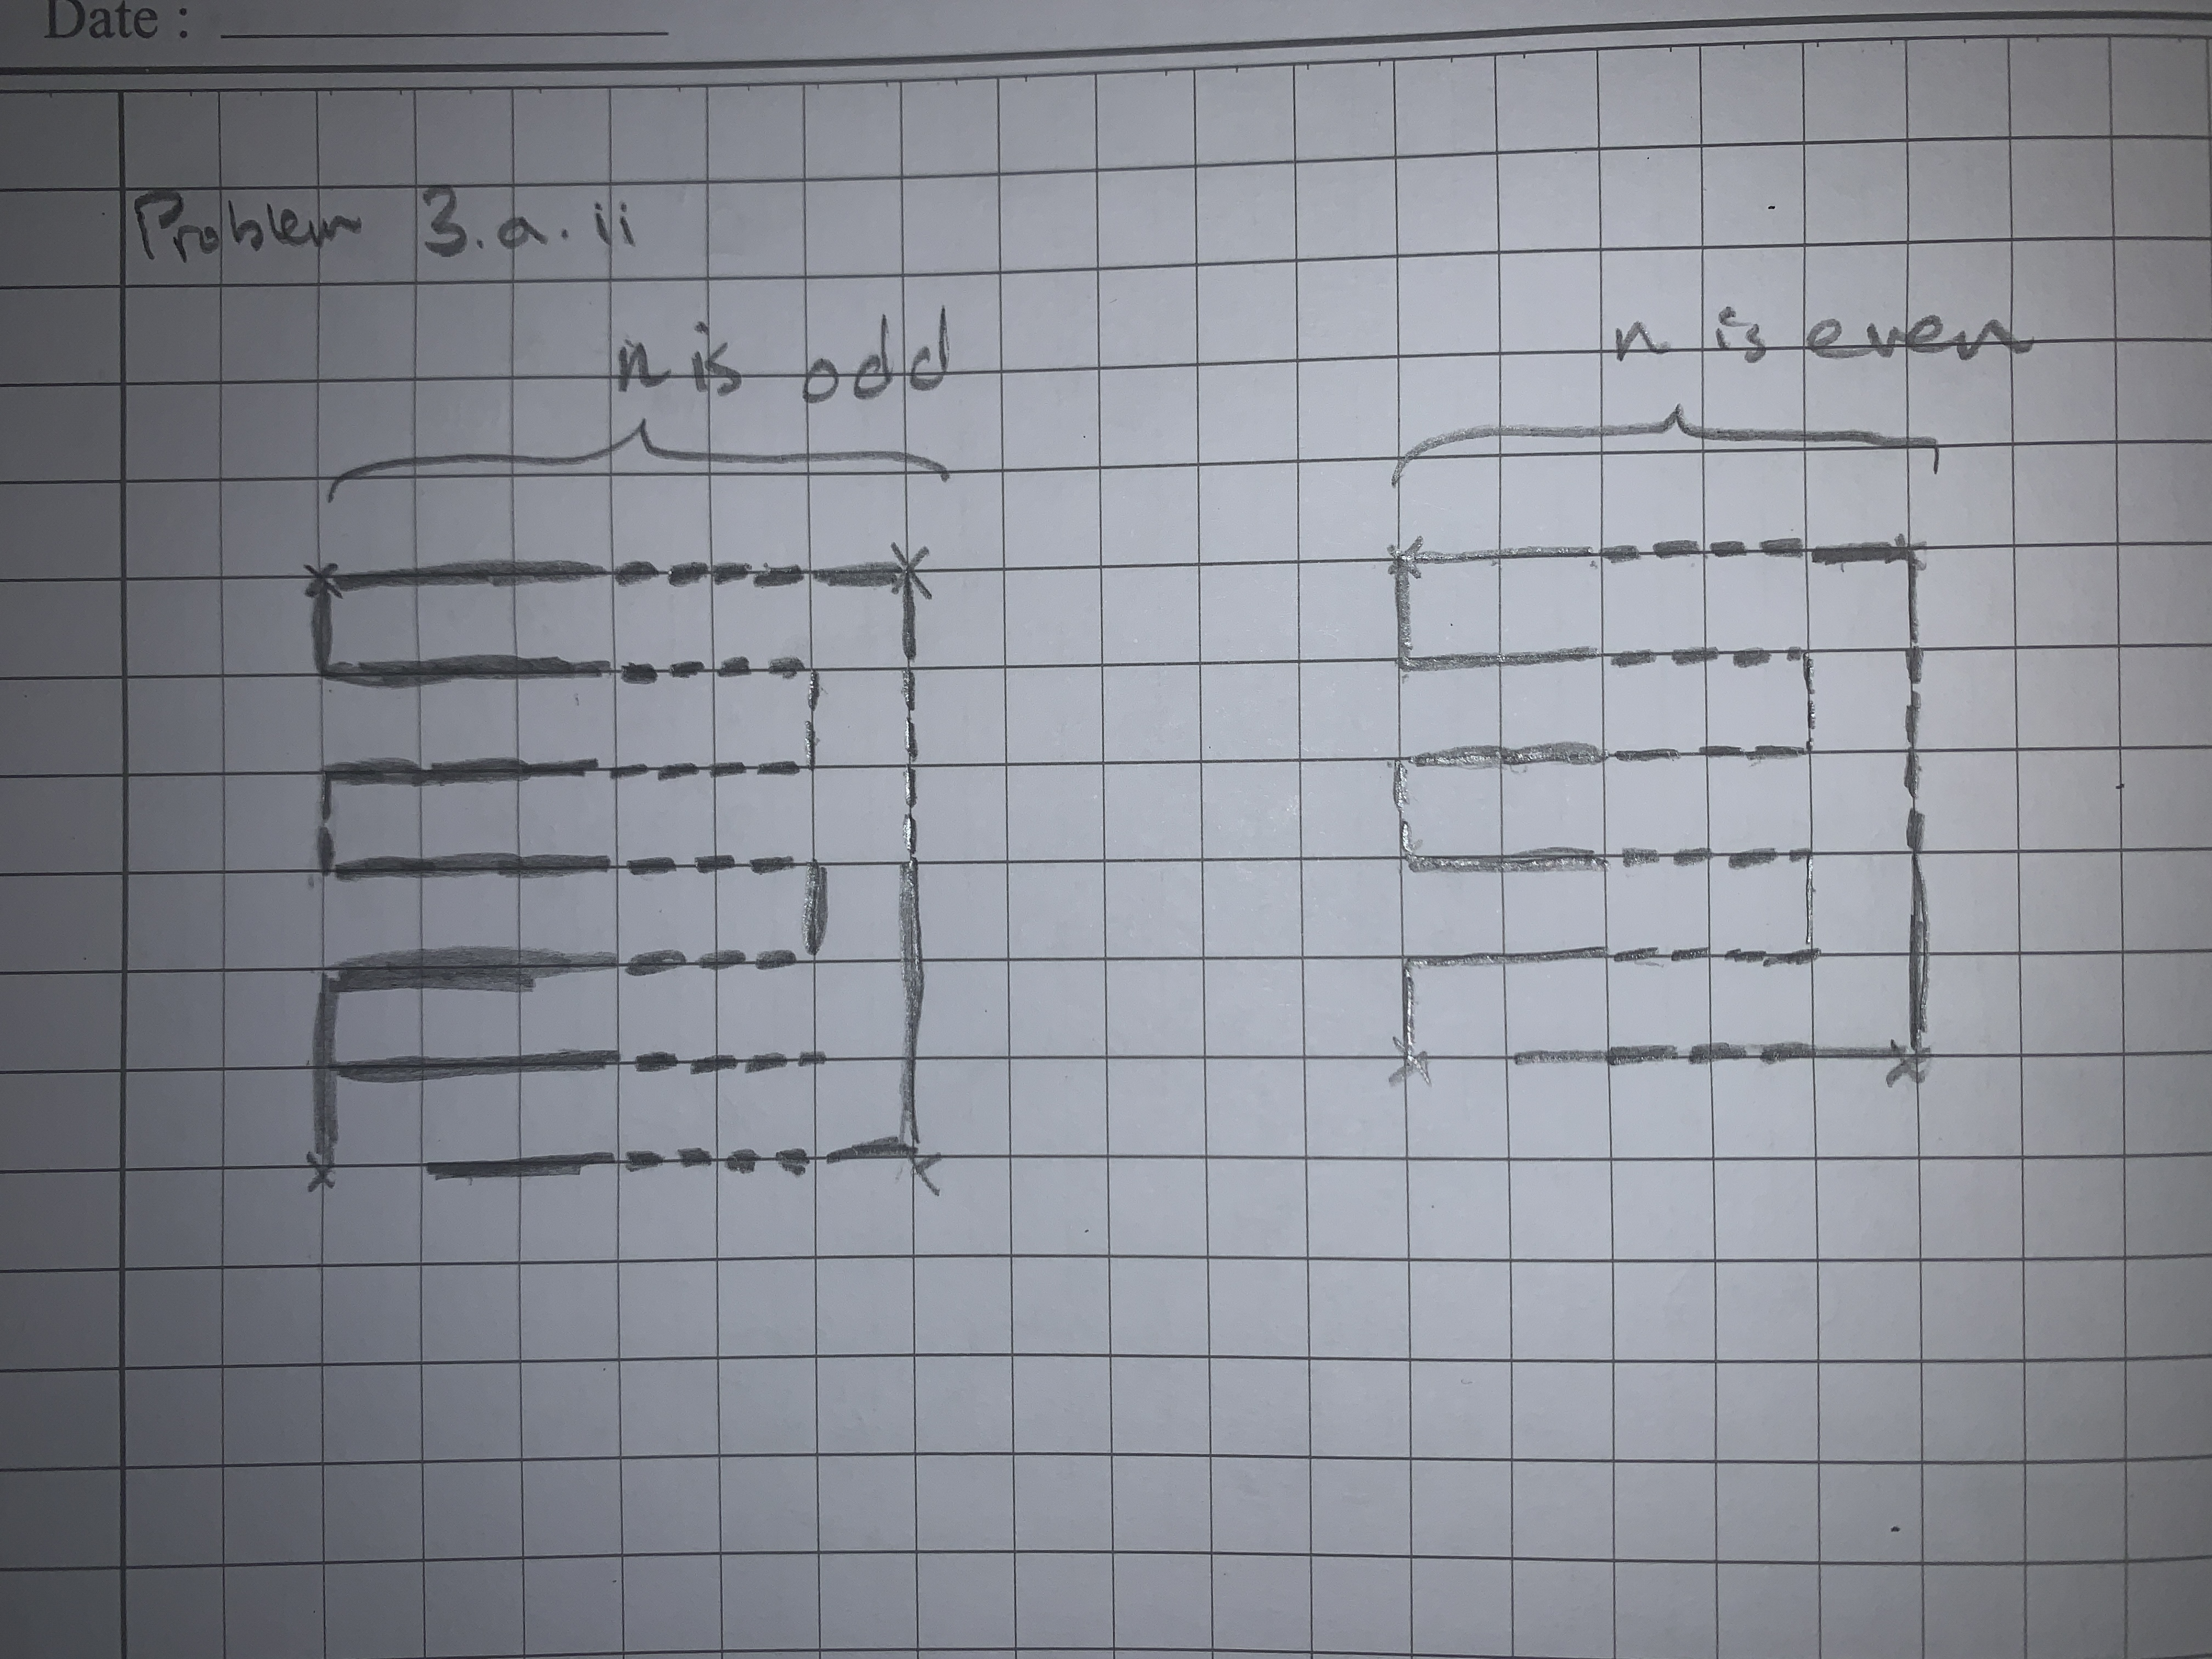
\includegraphics[width=0.8\textwidth]{p3-a-ii}
				\centering
			\end{figure}

		\end{enumerate}

		\item 
		\begin{enumerate}[label=(\roman*)]
			\item 
			\begin{align*}
				&\{(0, 0) - (1, 0) - \cdots - (n-1, 0)\}
					&\text{Base.} \\
				&\cup \{(i, 0) - (i, 1) - \cdots - (i, n-1) \mid 1 \le i \le n - 1\}
					&\text{V lines.} \\
				&\cup \{(0, j) - (1, j) \mid 1 \le j \le n - 1\}
					&\text{H lines.} \\
			\end{align*}

			\item \-
			\begin{figure}[H]
				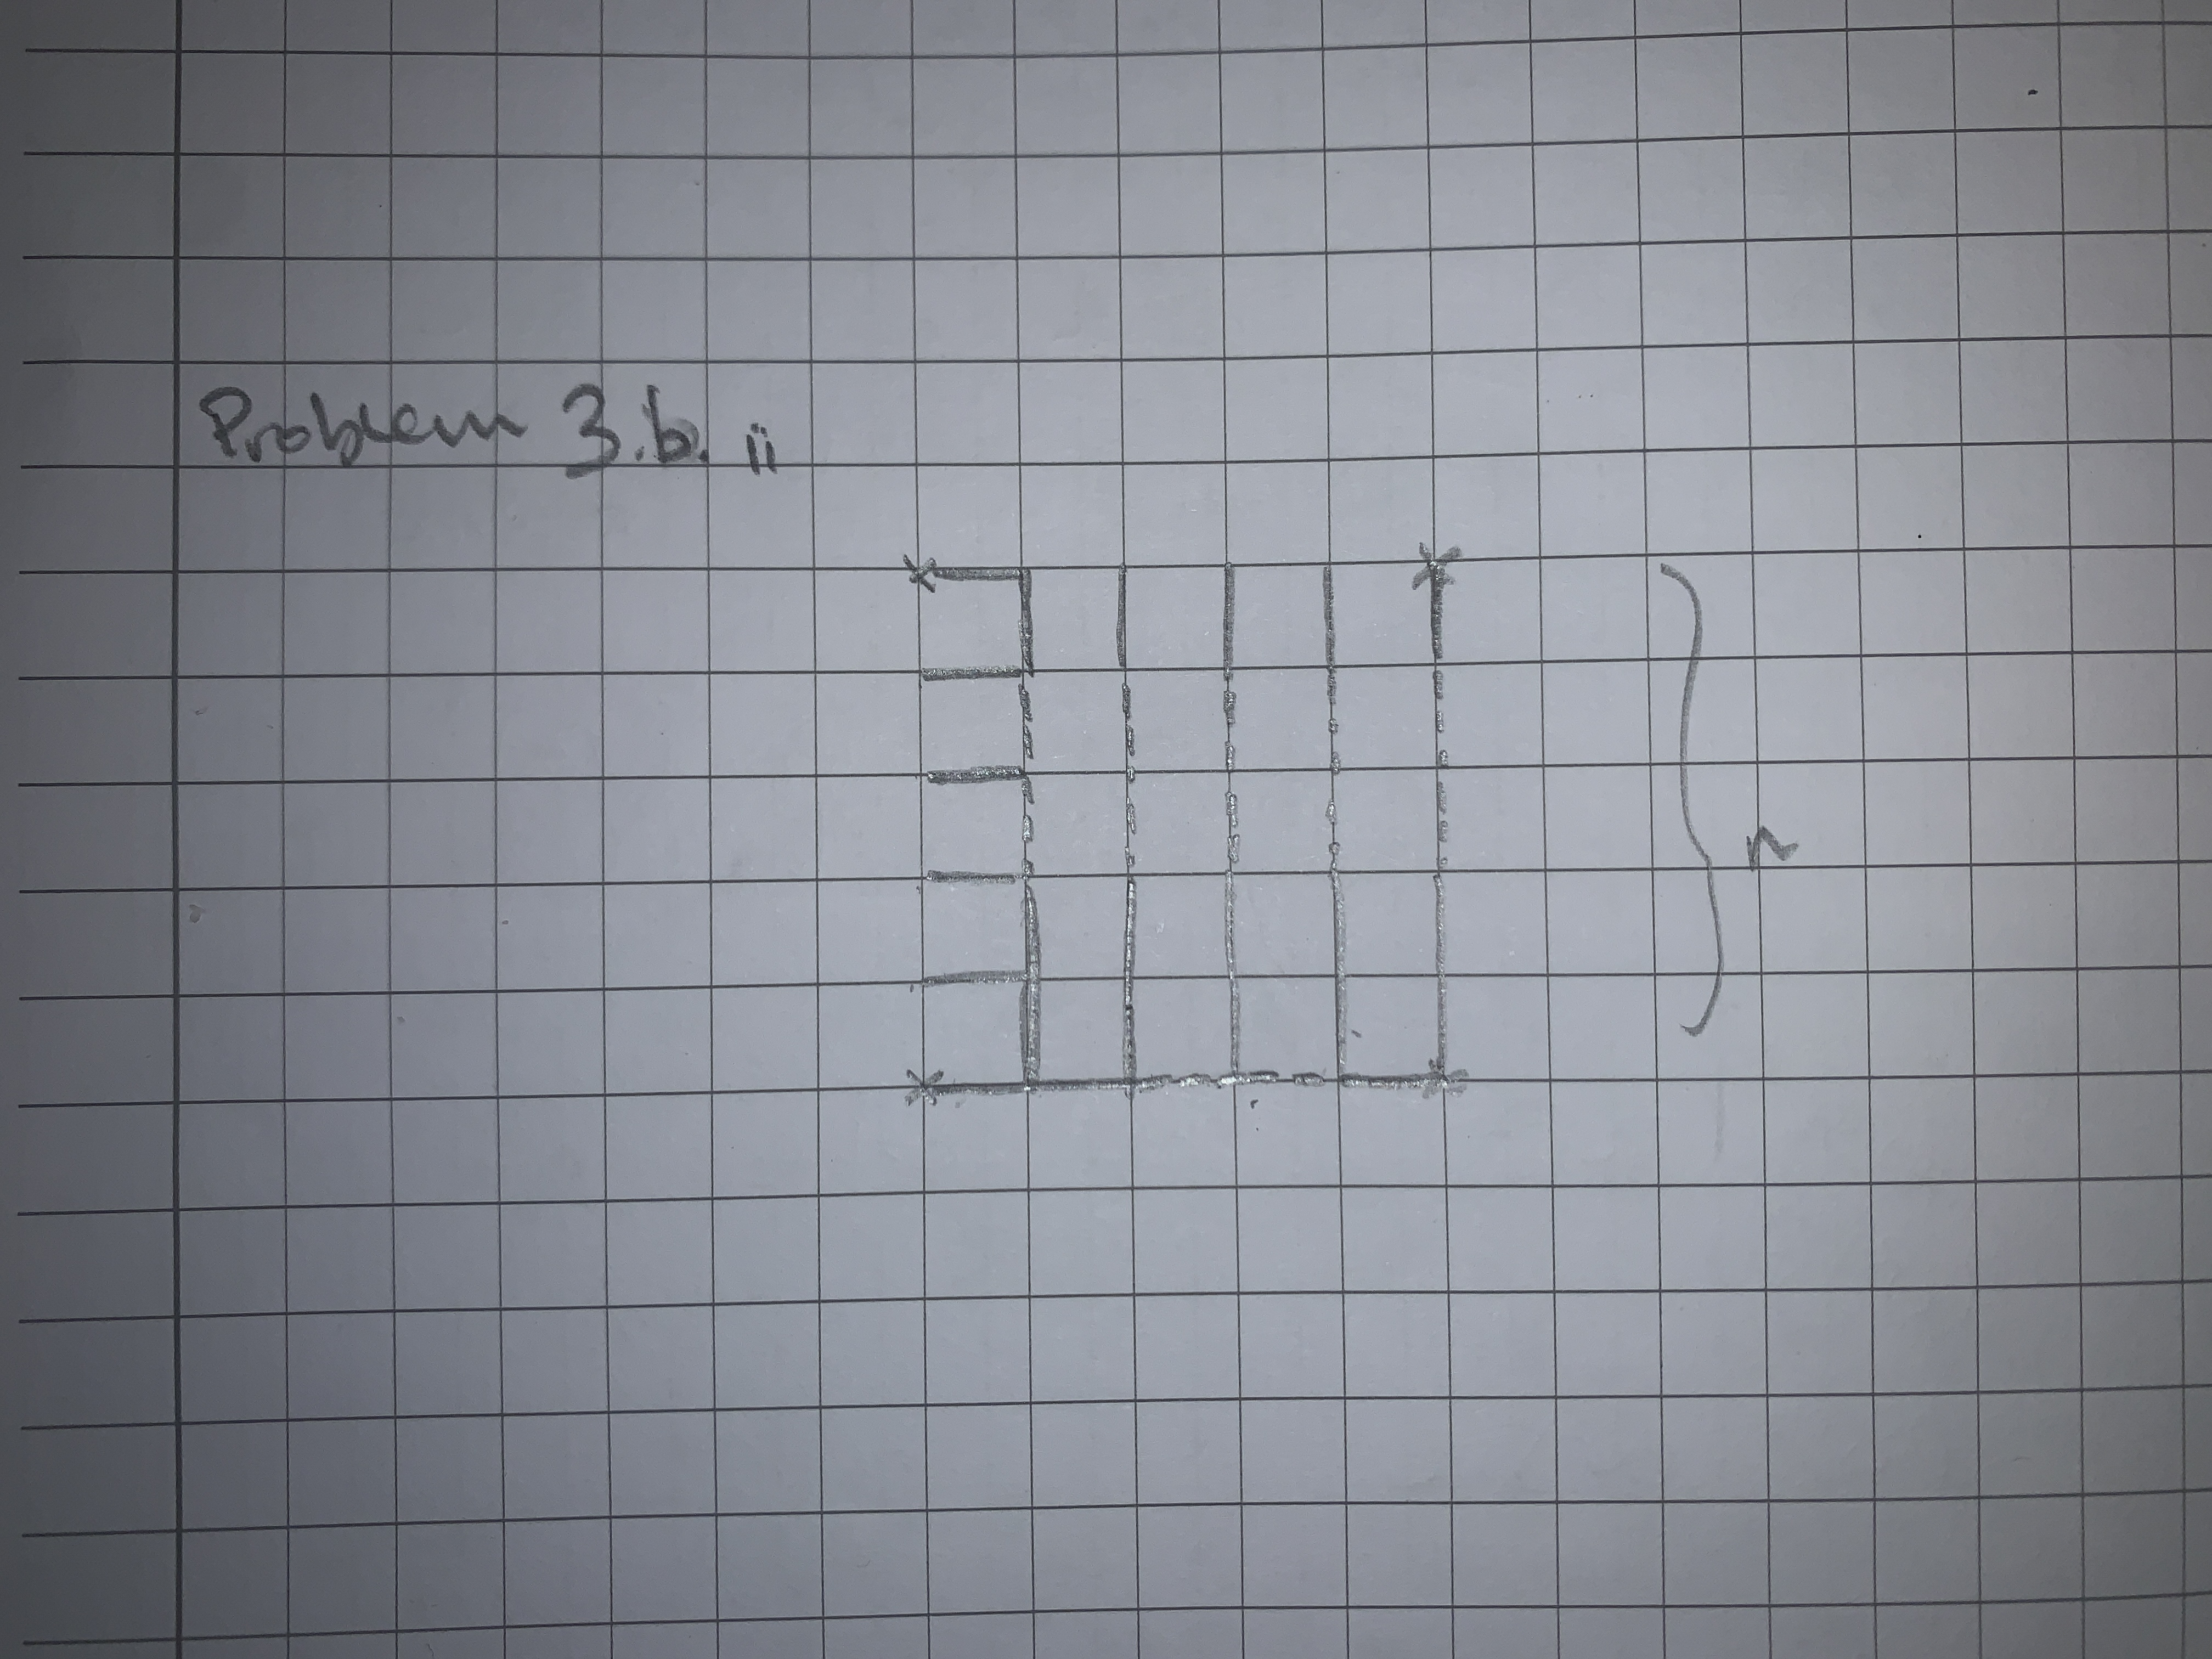
\includegraphics[width=0.8\textwidth]{p3-b-ii}
				\centering
			\end{figure}

		\end{enumerate}
		
	\end{enumerate} 


\newpage
\section*{Problem 4}
	\begin{enumerate}[label=(\Alph*)]
		\item \-
		\begin{figure}[H]
			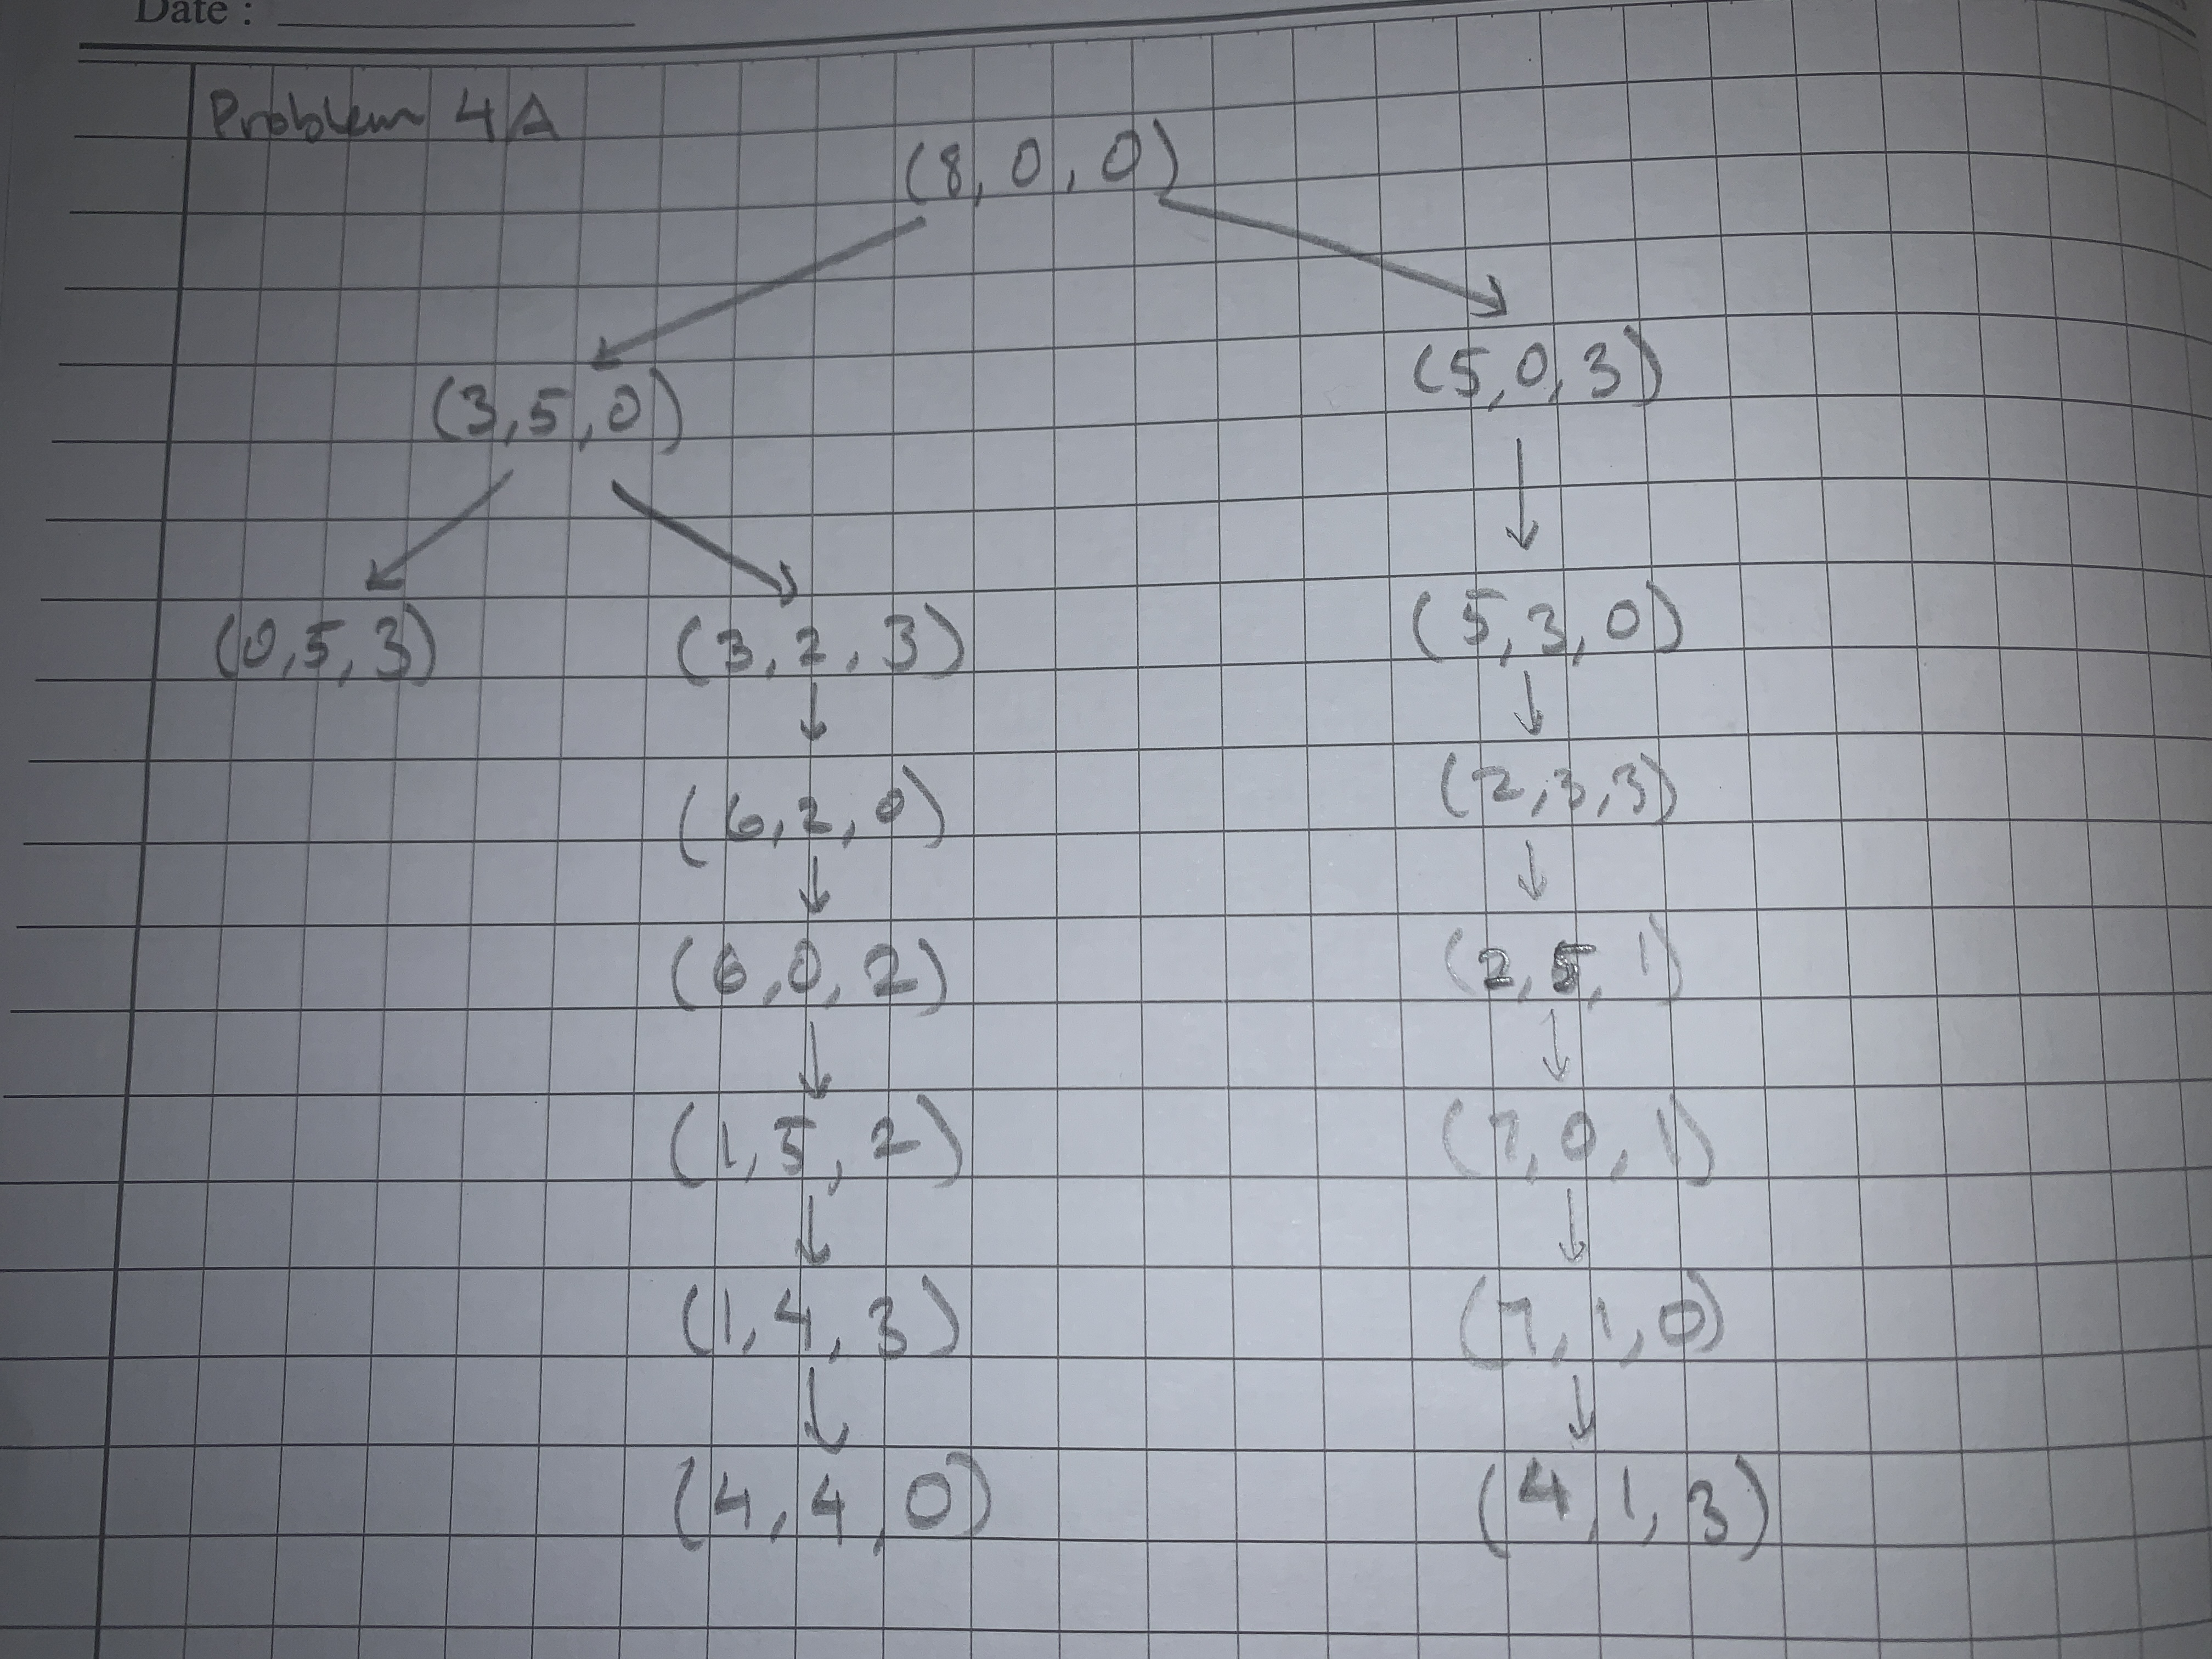
\includegraphics[width=0.8\textwidth]{p4-a}
			\centering
		\end{figure}
		
		\item \-
		\begin{figure}[H]
			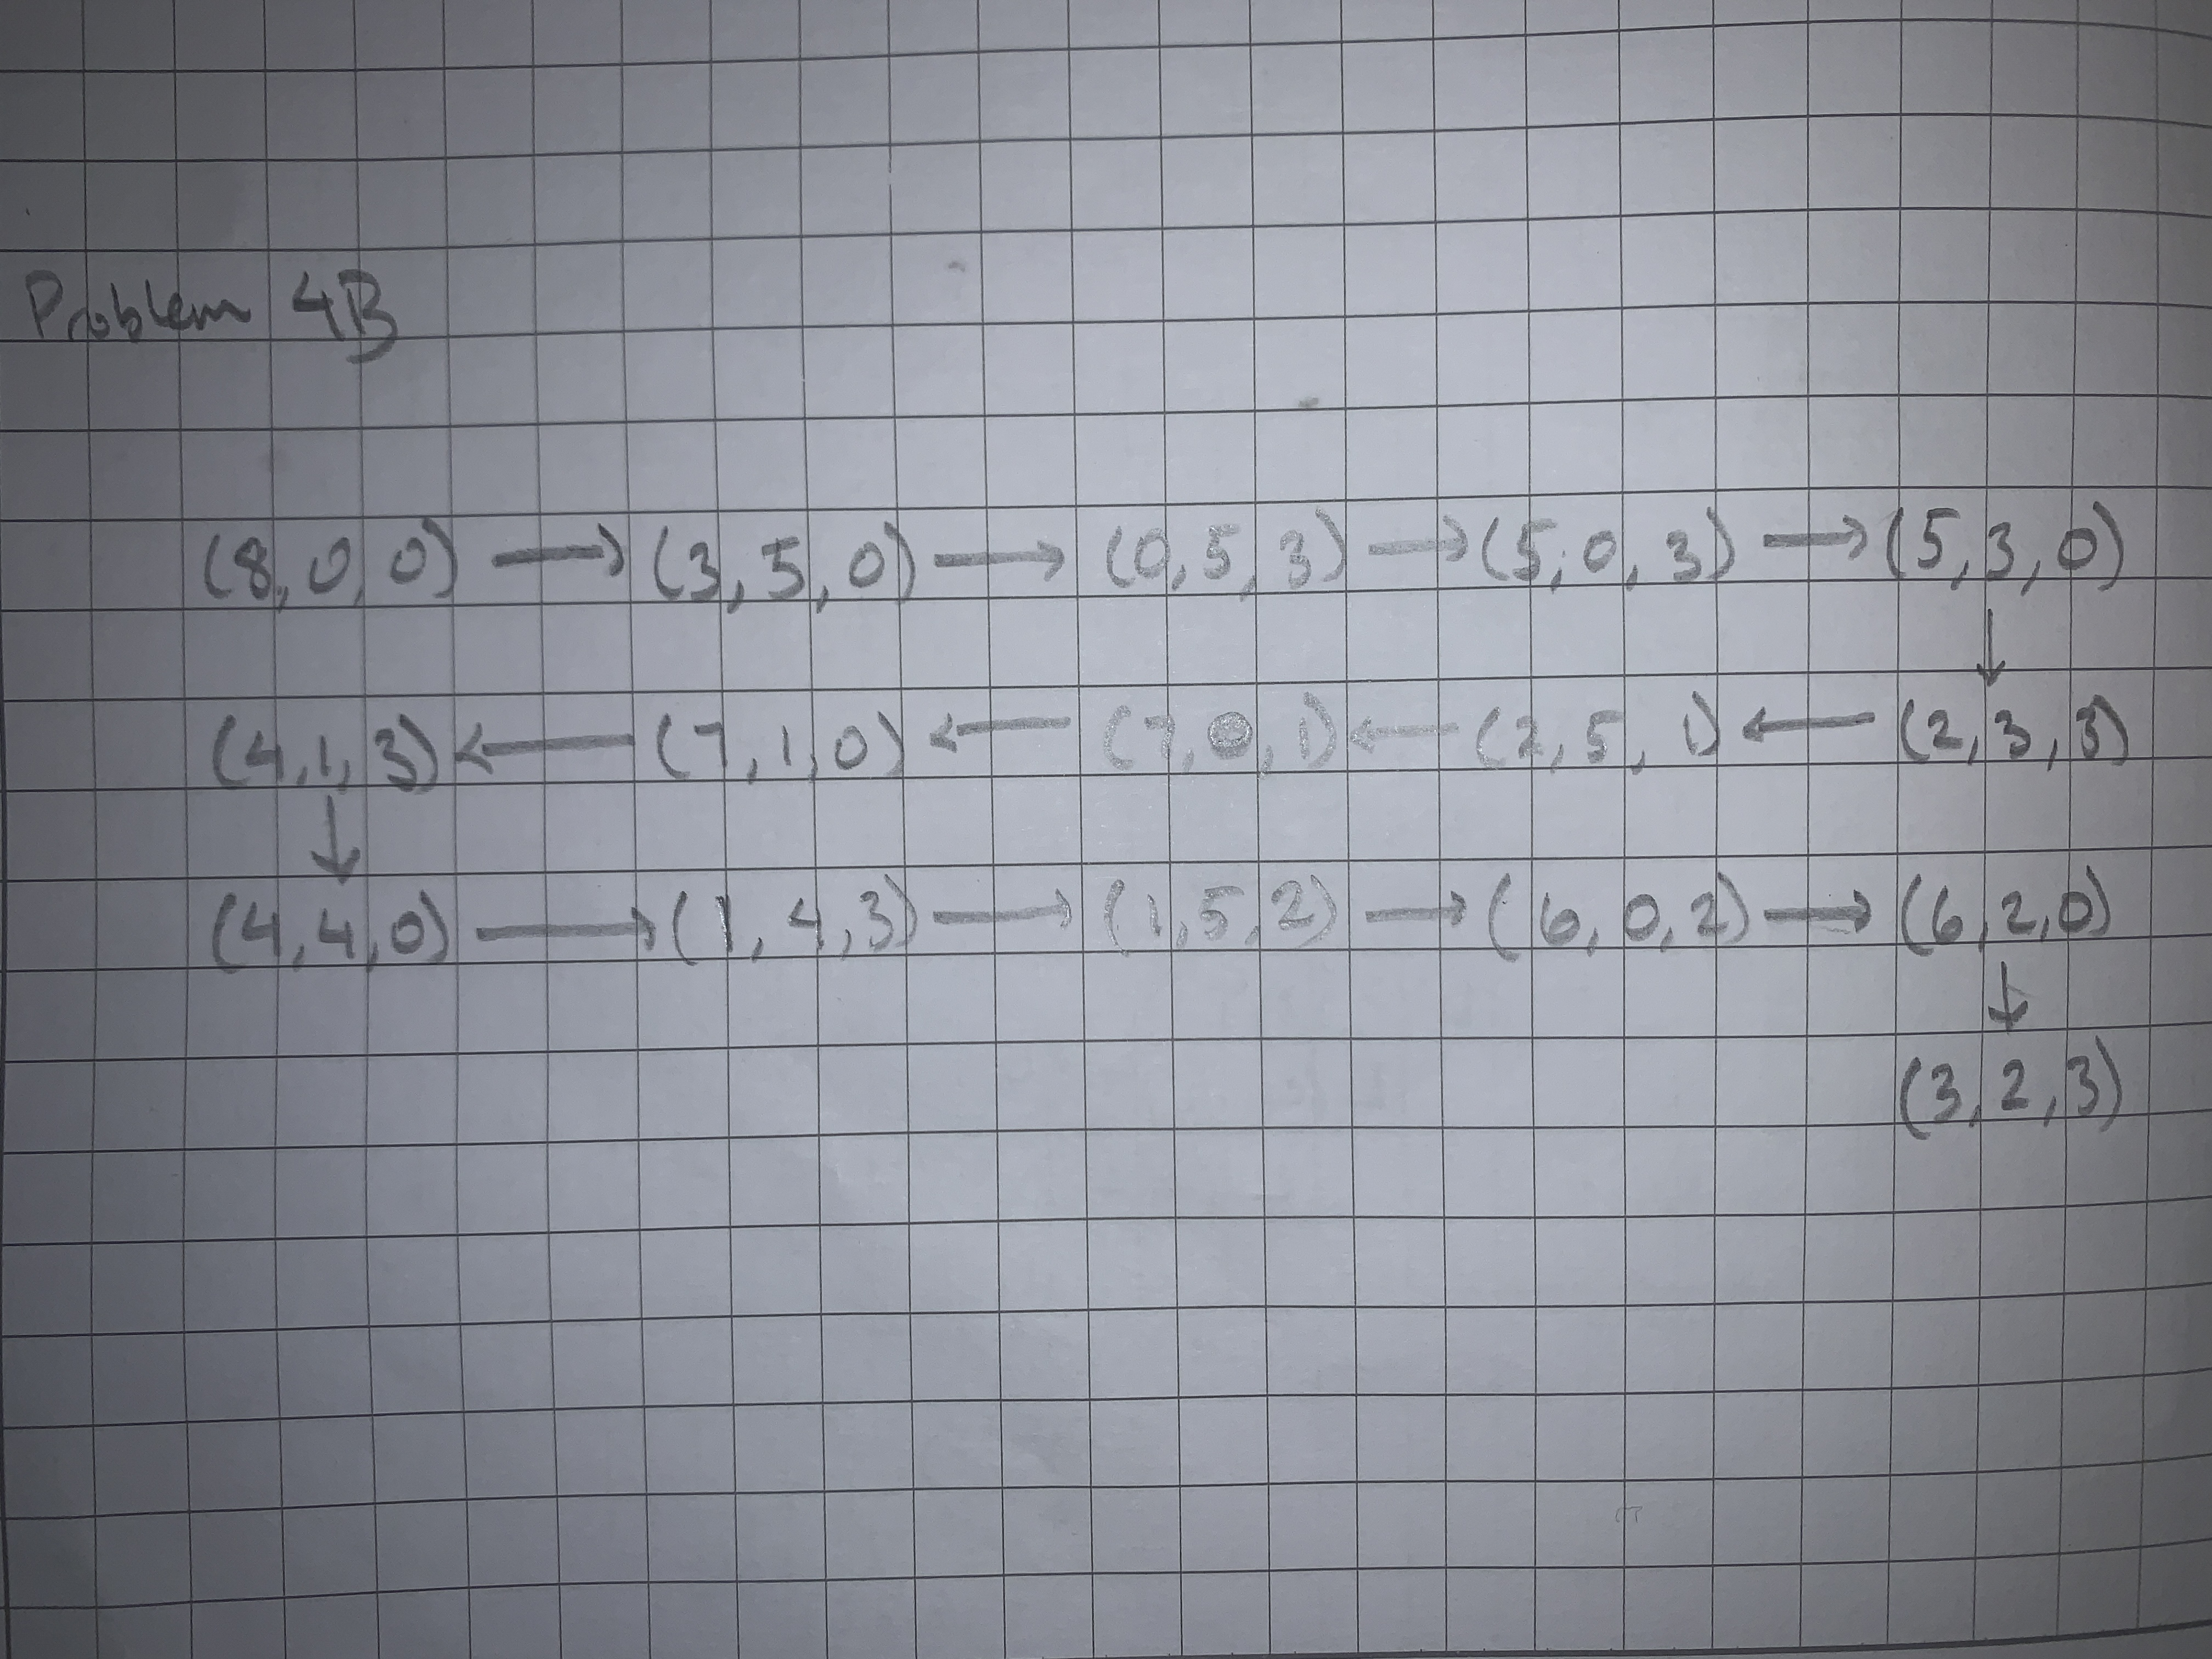
\includegraphics[width=0.8\textwidth]{p4-b}
			\centering
		\end{figure}

		\item Yes. BFS is a method to find a sequence of water pouring using the least number of pouring steps.
		
		\item
		Since the problem is modelled as an unweighted graph, BFS indiscriminately searches the graph in a radial search pattern (see (A)).
		
		Further nodes are not visited until all closer nodes have been visited. BFS uses a queue to ensure that nodes are visited by distance.\footnote{Distance meaning the length of the shortest path between two nodes.}

		\item No.
		\item No such sequence exists. This can be shown by performing BFS or DFS on the starting node (8, 0, 0) and exhausting all possible nodes (see (A) or (B)). No (6, 1, 1) node is connected to the graph of (8, 0, 0).
		
		\item For any $v \in V - \{v_0\}$, we can simply perform moves (iii) and (v) (i.e. moving water from $b$ or $c$ to $a$) to return to $v_0 = (8, 0, 0)$.

		\item A counterexample is sufficient to disprove the statement. $v_0$ is reachable from $(6, 1, 1)$ (use moves (iii) and (v)), but $(6, 1, 1)$ is not reachable from $v_0$.


	\end{enumerate}



\newpage
\section*{Problem 5}
	\begin{enumerate}[label=(\alph*)]
		\item 
		\begin{minipage}{0.53\linewidth}
			\begin{tabular}{|c||c|c|c|c|c|c|c|c|}
				\hline
				i/j & 1 & 2 & 3 & 4 & 5 & 6 & 7 & 8 \\\hline\hline
				1 	& 5 & 25& 35& 50& 85&110&160&175\\\hline
				2 	& 	& 15& 25& 40& 70& 95&145&160\\\hline
				3 	& 	&  	& 5 & 15& 35& 55&105&115\\\hline
				4 	& 	& 	& 	& 5 & 20& 40& 85& 95\\\hline
				5 	& 	& 	& 	& 	& 10& 30& 70& 80\\\hline
				6 	& 	& 	& 	& 	& 	& 10& 40& 50\\\hline
				7 	& 	& 	& 	& 	& 	& 	& 20& 30\\\hline
				8 	& 	& 	& 	& 	& 	& 	& 	& 5 \\\hline
			\end{tabular}
		\end{minipage}
		\begin{minipage}{0.45\linewidth}
			\begin{tabular}{|c||c|c|c|c|c|c|c|c|}
				\hline
				i/j & 1 & 2 & 3 & 4 & 5 & 6 & 7 & 8 \\\hline\hline
				1 	& 1 & 2	& 2	& 2	& 2	& 2	& 5	& 5\\\hline
				2 	& 	& 2	& 2	& 2	& 2	& 5	& 5	& 5\\\hline
				3 	& 	& 	& 3	& 3	& 4	& 5	& 5	& 7\\\hline
				4 	& 	& 	& 	& 4	& 5	& 5	& 6	& 7\\\hline
				5 	& 	& 	& 	& 	& 5	& 5	& 6	& 7\\\hline
				6 	& 	& 	& 	& 	& 	& 6	& 7	& 7\\\hline
				7 	& 	& 	& 	& 	& 	& 	& 7	& 7\\\hline
				8 	& 	& 	& 	& 	& 	& 	& 	& 8\\\hline
			\end{tabular}
		\end{minipage}

		% i		1	2	3	4	5	6	7	8
		% w[i]	5	15	5	5	10  10  20 	5
		% Total: 75

		% Iteration 1.
		% e[1,2] = min( 15+20 , 5+20 ); w[1,2] = 20;   r[1,2] = 2
		% e[2,3] = min(  5+20 , 15+20 ); w[2,3] = 20;  r[2,3] = 2
		% e[3,4] = min( 5+10, 5+10 ); r[3,4] = 3
		% e[4,5] = min(10, 5) + 15; r[4,5] = 5
		% e[5,6] = min(10, 10) + 20; r[5,6] = 5
		% e[6,7] = min(20, 10) + 30; r[6,7] = 7
		% e[7,8] = min(5,20) + 25; r[7,8] = 7

		\item Cost: 175
		
		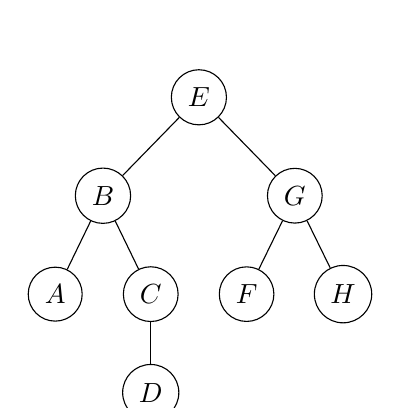
\begin{tikzpicture}[every tree node/.style={draw,circle},
			level distance=1.25cm,sibling distance=.5cm, 
			edge from parent path={(\tikzparentnode) -- (\tikzchildnode)}]
		\Tree [.{$E$}
			[.{$B$}
				[.{$A$}
				]
				[.{$C$}
					[.{$D$}
					]
				]
			]
			[.{$G$}
				[.{$F$}
				]
				[.{$H$}
				]
			]
		]
		\end{tikzpicture}

	\end{enumerate}


\end{document}